\chapter{Atividade 7 -- Escopo de variáveis e estratégias de escalonamento em OpenMP}
\label{chap:atvd07}


% ============================================================
\section{Enunciado da tarefa}
\label{sec:atvd07-enunciado}

\begin{quote}
Implemente diferentes versões de um programa para calcular quantos números
primos existem entre 2 e um valor máximo \(n\). O programa deve ser
paralelizado utilizando OpenMP.

Devem ser implementadas versões com a variável do contador utilizando apenas
\texttt{private}, apenas \texttt{firstprivate}, apenas
\texttt{lastprivate}, \texttt{firstprivate} e \texttt{lastprivate},
uso de \texttt{default(none)} e uma versão paralela utilizando
\texttt{reduction}.

A partir da versão selecionada como a de melhor comportamento, implemente
versões considerando os escalonadores \texttt{static}, \texttt{dynamic},
\texttt{guided}, \texttt{auto} e \texttt{runtime}. Analise os tempos médios
de execução de cada versão à medida que \(n\) aumenta e utilize gráficos
para apresentar e analisar os resultados.
\end{quote}


% ============================================================
\section{Objetivos e requisitos}
\label{sec:atvd07-objetivos}

A atividade teve como objetivo aprofundar dois aspectos fundamentais da
programação paralela com OpenMP: o escopo de variáveis em regiões paralelas
e a distribuição das iterações de um laço entre as threads.

O problema computacional foi mantido em continuidade com a Atividade 5:
determinar a quantidade de números primos existentes no intervalo

\[
[2,n].
\]

Essa continuidade permitiu reutilizar uma implementação previamente
validada e concentrar o experimento nos novos mecanismos do OpenMP.

Os objetivos específicos foram:

\begin{itemize}
    \item reutilizar o algoritmo de contagem de primos desenvolvido na
    Atividade 5;

    \item preservar a mesma função de teste de primalidade em todas as
    versões;

    \item analisar o comportamento das cláusulas
    \texttt{private},
    \texttt{firstprivate},
    \texttt{lastprivate},
    \texttt{firstprivate + lastprivate},
    \texttt{default(none)} e
    \texttt{reduction};

    \item verificar quais dessas construções preservam a contagem global
    correta;

    \item selecionar uma implementação paralela funcionalmente correta para
    o experimento de escalonamento;

    \item comparar as políticas
    \texttt{static},
    \texttt{dynamic},
    \texttt{guided},
    \texttt{auto} e
    \texttt{runtime};

    \item medir o tempo médio de execução das diferentes versões;

    \item manter fixos os demais parâmetros experimentais para isolar o
    efeito das cláusulas estudadas;

    \item representar os resultados por meio de tabelas e gráficos;

    \item discutir correção, sincronização, overhead e balanceamento de
    carga.
\end{itemize}

A atividade foi estruturada em dois experimentos principais:

\begin{enumerate}
    \item comparação das cláusulas de escopo de dados;
    \item comparação das estratégias de escalonamento utilizando
    \texttt{reduction}.
\end{enumerate}


% ============================================================
\section{Fundamentação conceitual}
\label{sec:atvd07-fundamentacao}

\subsection{Paralelismo na contagem de números primos}

A contagem considera todos os candidatos pertencentes ao intervalo

\[
2,3,\ldots,n.
\]

Para cada candidato \(x\), é realizada uma classificação independente:

\[
P(x)=
\begin{cases}
1, & \text{se } x \text{ é primo},\\
0, & \text{caso contrário}.
\end{cases}
\]

A quantidade total de números primos é, portanto,

\[
C(n)=\sum_{x=2}^{n}P(x).
\]

Como a classificação de um candidato não depende dos demais, o laço que
percorre os candidatos apresenta paralelismo de dados natural.

O desafio está na agregação das contribuições individuais para o contador
global.


\subsection{Variáveis compartilhadas e privadas}

Em uma região paralela OpenMP, as threads podem acessar variáveis com
diferentes regras de compartilhamento.

Uma variável compartilhada possui uma única instância visível pelas
threads, enquanto uma variável privada possui uma instância independente
para cada thread.

Essa distinção é fundamental para a contagem de primos. Embora o trabalho
de testar os candidatos seja independente, a contagem final representa uma
operação global:

\[
C=C_0+C_1+\cdots+C_{T-1},
\]

onde \(C_i\) representa a quantidade encontrada pela thread \(i\).

A simples criação de cópias privadas não realiza automaticamente essa soma.


\subsection{\texttt{private}}

A cláusula

\begin{verbatim}
private(count)
\end{verbatim}

cria uma cópia independente de \texttt{count} para cada thread.

As cópias por thread são representadas na Figura~\ref{fig:atvd07-private}.

\begin{figure}[htbp]
    \centering
    \begin{tikzpicture}[node distance=0.6cm and 0.45cm, font=\small]
        \node[componente, text width=3.4cm] (shared)
            {Variável externa\\\texttt{count}};
        \node[processo, right=1.1cm of shared, text width=3.5cm] (clause)
            {\texttt{private(count)}};
        \node[thread, below left=of clause, text width=2.4cm] (t0)
            {Thread 0\\cópia privada};
        \node[thread, below=of clause, text width=2.4cm] (t1)
            {Thread 1\\cópia privada};
        \node[thread, below right=of clause, text width=2.4cm] (t2)
            {Thread \(T-1\)\\cópia privada};
        \node[componente, below=0.9cm of t1, text width=4.2cm] (discard)
            {Cópias descartadas\\sem soma global};
        \draw[fluxo] (shared) -- (clause);
        \draw[fluxo] (clause) -- (t0);
        \draw[fluxo] (clause) -- (t1);
        \draw[fluxo] (clause) -- (t2);
        \draw[fluxo] (t0) |- (discard);
        \draw[fluxo] (t1) -- (discard);
        \draw[fluxo] (t2) |- (discard);
    \end{tikzpicture}
    \caption{Cópias privadas independentes sem agregação ao contador externo.}
    \label{fig:atvd07-private}
\end{figure}

As cópias privadas não recebem automaticamente o valor anteriormente
armazenado na variável original e também não são automaticamente combinadas
ao término da região paralela.

Assim,

\[
\texttt{private}
\]

resolve o isolamento entre as threads, mas não resolve a agregação das
contagens.


\subsection{\texttt{firstprivate}}

A cláusula

\begin{verbatim}
firstprivate(count)
\end{verbatim}

também cria uma cópia privada para cada thread, mas inicializa essa cópia
com o valor existente antes da região paralela.

Se inicialmente

\[
count=0,
\]

então todas as threads começam com

\[
count_i=0.
\]

Ao final da região, entretanto, essas cópias continuam sendo descartadas.

Portanto,

\[
\texttt{firstprivate}
\]

resolve a inicialização das cópias, mas não implementa uma operação de
redução.


\subsection{\texttt{lastprivate}}

A cláusula

\begin{verbatim}
lastprivate(count)
\end{verbatim}

torna a variável privada durante o laço e, ao término da região paralela,
transfere para a variável externa o valor correspondente à última iteração
lógica do laço.

Isso não representa a soma das contribuições das threads.

Formalmente,

\[
\texttt{lastprivate}
\neq
\sum_i C_i.
\]

Existe ainda um cuidado importante: a cópia privada criada por
\texttt{lastprivate} não deve ser lida sem inicialização.

Na implementação desta atividade, \texttt{count} é explicitamente definido
antes de ser utilizado em cada iteração, evitando leitura de valor
indeterminado.


\subsection{\texttt{firstprivate} e \texttt{lastprivate}}

A combinação

\begin{verbatim}
firstprivate(count) lastprivate(count)
\end{verbatim}

faz com que cada cópia privada seja inicializada com o valor externo e que,
ao final, a cópia associada à última iteração lógica seja propagada para a
variável externa.

Entretanto, continua não existindo uma agregação global.

Assim,

\[
\boxed{
\texttt{firstprivate + lastprivate}
\neq
\texttt{reduction}
}
\]


\subsection{\texttt{default(none)}}

A cláusula

\begin{verbatim}
default(none)
\end{verbatim}

obriga que o programador declare explicitamente a classificação das
variáveis utilizadas na região paralela.

Seu objetivo é aumentar a clareza da política de compartilhamento e reduzir
erros decorrentes de classificações implícitas.

Entretanto,

\[
\boxed{
\texttt{default(none)}
\text{ não é um mecanismo de sincronização}
}
\]

Se uma variável for explicitamente declarada como compartilhada e múltiplas
threads realizarem atualizações concorrentes sem proteção, a condição de
corrida continua existindo.


\subsection{Condição de corrida}

A operação

\begin{verbatim}
++count;
\end{verbatim}

não deve ser interpretada como uma única operação indivisível.

Conceitualmente, ela envolve:

\begin{enumerate}
    \item leitura do valor;
    \item incremento;
    \item escrita do novo valor.
\end{enumerate}

Se duas ou mais threads realizarem essas operações simultaneamente sobre o
mesmo contador compartilhado, atualizações podem ser perdidas.

Essa situação constitui uma \textit{data race}.

Os resultados produzidos por uma implementação com condição de corrida não
possuem garantia de correção e uma eventual coincidência com o resultado
esperado não elimina o erro de sincronização.


\subsection{\texttt{reduction}}

O padrão matemático da contagem de primos é uma soma de resultados
parciais.

OpenMP fornece diretamente esse padrão por meio de:

\begin{verbatim}
reduction(+:count)
\end{verbatim}

Cada thread realiza sua própria acumulação e, ao final da região, OpenMP
combina os valores privados.

O processo de combinação é ilustrado na Figura~\ref{fig:atvd07-reduction}.

\begin{figure}[htbp]
    \centering
    \begin{tikzpicture}[node distance=0.55cm and 0.55cm, font=\small]
        \node[thread, text width=2.4cm] (t0) {Thread 0\\soma privada \(C_0\)};
        \node[thread, right=of t0, text width=2.4cm] (t1) {Thread 1\\soma privada \(C_1\)};
        \node[thread, right=of t1, text width=2.4cm] (tt) {Thread \(T-1\)\\soma privada \(C_{T-1}\)};
        \node[processo, below=of t1, text width=4.0cm] (combine)
            {Combinar\\\texttt{reduction(+:count)}};
        \node[componente, below=of combine, text width=3.2cm] (total)
            {Contagem global\\\(C=\sum_i C_i\)};
        \draw[fluxo] (t0) -- (combine);
        \draw[fluxo] (t1) -- (combine);
        \draw[fluxo] (tt) -- (combine);
        \draw[fluxo] (combine) -- (total);
    \end{tikzpicture}
    \caption{Agregação das contagens privadas pela cláusula \texttt{reduction}.}
    \label{fig:atvd07-reduction}
\end{figure}

Assim,

\[
C=\sum_{i=0}^{T-1}C_i.
\]

A cláusula representa diretamente a operação necessária para obter a
contagem global.


\subsection{Escalonamento de iterações}

Depois de definida uma implementação paralela correta, é necessário decidir
como as iterações do laço serão distribuídas entre as threads.

Em OpenMP essa política pode ser especificada por meio da cláusula
\texttt{schedule}.


\subsubsection{\texttt{static}}

Na política

\begin{verbatim}
schedule(static)
\end{verbatim}

as iterações são distribuídas previamente entre as threads.

Essa abordagem possui baixo overhead e comportamento previsvisível.

Entretanto, uma quantidade semelhante de iterações não implica
necessariamente uma quantidade semelhante de trabalho.


\subsubsection{\texttt{dynamic}}

Na política

\begin{verbatim}
schedule(dynamic)
\end{verbatim}

novos blocos de iterações são obtidos pelas threads à medida que o trabalho
anterior é concluído.

Isso pode melhorar o balanceamento de cargas irregulares, mas aumenta o
custo de gerenciamento do escalonamento.


\subsubsection{\texttt{guided}}

Em

\begin{verbatim}
schedule(guided)
\end{verbatim}

o trabalho também é distribuído dinamicamente, mas blocos maiores são
utilizados inicialmente e seu tamanho é progressivamente reduzido.

A estratégia busca combinar:

\[
\text{baixo overhead inicial}
\]

com

\[
\text{melhor balanceamento próximo ao final}.
\]


\subsubsection{\texttt{auto}}

Com

\begin{verbatim}
schedule(auto)
\end{verbatim}

a escolha da forma de distribuição é delegada à implementação OpenMP.

O programa não determina explicitamente qual estratégia interna será
utilizada.


\subsubsection{\texttt{runtime}}

Com

\begin{verbatim}
schedule(runtime)
\end{verbatim}

a configuração do escalonamento é determinada em tempo de execução.

Nesta atividade, a política foi explicitamente configurada como

\[
\texttt{dynamic},\quad chunk=1.
\]

Dessa forma, o significado de \texttt{runtime} permaneceu reproduzível
durante o experimento.


\subsection{Irregularidade da carga}

O custo do teste de primalidade não é uniforme.

Números pares são rejeitados imediatamente, enquanto candidatos ímpares,
especialmente números primos maiores, podem exigir vários testes de
divisibilidade.

Assim,

\[
W(i)\neq W(j),
\]

onde \(W(x)\) representa o trabalho necessário para testar o candidato
\(x\).

Essa característica torna o problema apropriado para avaliar políticas de
escalonamento.


\subsection{Tempo médio}

O enunciado solicita a análise do tempo médio de execução.

Para \(M=20\) medições,

\[
T_{\mathrm{medio}}
=
\frac{1}{20}
\sum_{i=1}^{20}T_i.
\]

Essa estatística foi utilizada como medida principal nesta atividade.


% ============================================================
\section{Interpretação didática da tarefa}
\label{sec:atvd07-interpretacao}

A atividade foi interpretada como uma continuação direta do estudo iniciado
na Atividade 5.

Na atividade anterior, verificou-se que uma simples paralelização do laço
com um contador compartilhado produzia uma condição de corrida e que a
cláusula \texttt{reduction} fornecia a agregação correta.

Nesta atividade, o objetivo foi decompor esse problema em duas questões.

A primeira foi:

\begin{quote}
Como diferentes cláusulas de escopo alteram o comportamento de uma variável
utilizada como contador?
\end{quote}

A segunda foi:

\begin{quote}
Depois de obtida uma implementação correta, como a política utilizada para
distribuir as iterações influencia o desempenho?
\end{quote}

Assim, a progressão didática adotada está representada na
Figura~\ref{fig:atvd07-percurso}.

\begin{figure}[htbp]
    \centering
    \begin{tikzpicture}[node distance=0.45cm and 0.45cm, font=\small]
        \node[processo, text width=4.4cm] (seq) {Contagem sequencial};
        \node[componente, below=of seq, text width=4.4cm] (scope)
            {Investigar escopo de dados};
        \node[thread, below left=of scope, text width=2.7cm] (private)
            {\texttt{private}, \texttt{firstprivate},\\\texttt{lastprivate} e combinação};
        \node[thread, below=of scope, text width=2.7cm] (default)
            {\texttt{default(none)}};
        \node[thread, below right=of scope, text width=2.7cm] (reduction)
            {\texttt{reduction}};
        \node[componente, below=0.8cm of default, text width=3.8cm] (check)
            {Validar resultados};
        \node[decisao, below=of check, text width=3.2cm] (valid)
            {Contagem correta?};
        \node[componente, right=1.2cm of valid, yshift=-0.7cm, text width=2.5cm] (discard)
            {Descartar versão incorreta};
        \node[processo, below=of valid, text width=4.4cm] (selected)
            {Selecionar \texttt{reduction}};
        \node[componente, below=of selected, text width=4.4cm] (schedule)
            {Comparar schedules\\static, dynamic, guided, auto, runtime};
        \node[processo, below=of schedule, text width=4.4cm] (performance)
            {Analisar desempenho};
        \draw[fluxo] (seq) -- (scope);
        \draw[fluxo] (scope) -- (private);
        \draw[fluxo] (scope) -- (default);
        \draw[fluxo] (scope) -- (reduction);
        \draw[fluxo] (private.south) |- (check.west);
        \draw[fluxo] (default.south) -- (check.north);
        \draw[fluxo] (reduction.south) |- (check.east);
        \draw[fluxo] (check) -- (valid);
        \draw[fluxo] (valid) -- node[right] {sim} (selected);
        \draw[fluxo] (valid.east) -- node[pos=0.5,above] {não} (discard.west);
        \draw[fluxo] (selected) -- (schedule);
        \draw[fluxo] (schedule) -- (performance);
    \end{tikzpicture}
    \caption{Progressão da análise de escopo até a comparação de desempenho.}
    \label{fig:atvd07-percurso}
\end{figure}

A atividade, portanto, separa explicitamente dois problemas que podem ser
confundidos em uma primeira abordagem à programação paralela:

\[
\boxed{\text{compartilhamento de dados}}
\]

e

\[
\boxed{\text{distribuição do trabalho}}.
\]


% ============================================================
\section{Modelagem da solução}
\label{sec:atvd07-modelagem}

\subsection{Estrutura geral}

A solução foi implementada por adaptação direta do programa desenvolvido na
Atividade 5.

Foram preservados:

\begin{itemize}
    \item o algoritmo de primalidade;
    \item os valores de \(N\);
    \item as contagens conhecidas de primos;
    \item a temporização baseada em \texttt{omp\_get\_wtime()};
    \item os aquecimentos;
    \item as repetições internas calibradas;
    \item a validação funcional;
    \item o uso de quatro threads.
\end{itemize}

A nova implementação foi dividida em dois experimentos.


\subsubsection{Experimento A -- Escopo de dados}

Foram consideradas sete implementações:

\begin{enumerate}
    \item sequencial;
    \item \texttt{private};
    \item \texttt{firstprivate};
    \item \texttt{lastprivate};
    \item \texttt{firstprivate + lastprivate};
    \item \texttt{default(none)};
    \item \texttt{reduction}.
\end{enumerate}

A versão sequencial foi utilizada como referência.

A seleção da implementação a ser utilizada posteriormente não foi baseada
apenas no menor tempo, mas na ordem:

\[
\boxed{
\text{correção}
\longrightarrow
\text{desempenho}
}
\]


\subsubsection{Experimento B -- Escalonamento}

A versão com \texttt{reduction}, validada no primeiro experimento, foi
utilizada como base.

A única dimensão modificada passou a ser a política de escalonamento:

\begin{enumerate}
    \item \texttt{static};
    \item \texttt{dynamic};
    \item \texttt{guided};
    \item \texttt{auto};
    \item \texttt{runtime}.
\end{enumerate}

Todas as versões continuaram utilizando exatamente o mesmo teste de
primalidade e a mesma redução.


\subsection{Principais funções e componentes}

A organização principal do programa é apresentada na
Tabela~\ref{tab:atvd07-componentes}.

\begin{table}[htbp]
\centering
\caption{Principais componentes da implementação da Atividade 7.}
\label{tab:atvd07-componentes}
\small
\begin{tabular}{|p{0.38\textwidth}|p{0.52\textwidth}|}
\hline
\textbf{Componente} & \textbf{Responsabilidade} \\
\hline
\texttt{is\_prime()} &
Teste de primalidade comum a todas as versões. \\
\hline

\texttt{count\_primes\_sequential()} &
Implementação sequencial de referência. \\
\hline

\texttt{count\_primes\_private()} &
Versão com cópias privadas do contador. \\
\hline

\texttt{count\_primes\_firstprivate()} &
Versão cujas cópias privadas recebem o valor inicial do contador. \\
\hline

\texttt{count\_primes\_lastprivate()} &
Versão que propaga o valor da última iteração lógica. \\
\hline

\texttt{count\_primes\_first\_lastprivate()} &
Combina inicialização privada e propagação da última iteração. \\
\hline

\texttt{count\_primes\_default\_none()} &
Declara explicitamente o compartilhamento, mantendo o contador
compartilhado sem sincronização. \\
\hline

\texttt{count\_primes\_reduction()} &
Implementação correta com redução e \texttt{schedule(static)}. \\
\hline

Funções de \texttt{schedule} &
Implementam \texttt{dynamic}, \texttt{guided}, \texttt{auto} e
\texttt{runtime}, sempre com redução. \\
\hline

\texttt{run\_timed\_batch()} &
Executa várias chamadas dentro de um único intervalo cronometrado. \\
\hline

\texttt{calibrate\_internal\_repetitions()} &
Determina um número comum de repetições internas por valor de \(N\). \\
\hline

\texttt{run\_warmups\_rotated()} &
Executa aquecimentos alterando a ordem inicial das versões. \\
\hline

\texttt{benchmark\_function\_set()} &
Executa vinte medições por versão, com ordem rotacionada, e calcula a
média. \\
\hline

Funções de exportação CSV &
Persistem os resultados utilizados na geração e análise dos gráficos. \\
\hline
\end{tabular}
\end{table}


% ============================================================
\section{Decisões de projeto e trade-offs}
\label{sec:atvd07-decisoes}

\subsection{Reutilização da Atividade 5}

A implementação não foi reconstruída do início.

O código anterior já fornecia:

\begin{itemize}
    \item teste de primalidade validado;
    \item valores conhecidos de referência;
    \item controle da quantidade de threads;
    \item temporização;
    \item aquecimentos;
    \item calibração de lotes;
    \item mecanismo para impedir a eliminação da computação pelo compilador.
\end{itemize}

A reutilização reduz a quantidade de novas variáveis introduzidas no
experimento e mantém continuidade entre as atividades.


\subsection{Mesma função de primalidade}

Todas as versões utilizam a mesma função \texttt{is\_prime()}.

Não foram introduzidos algoritmos alternativos, como crivos ou novas
otimizações específicas.

Assim, as diferenças observadas decorrem das construções OpenMP avaliadas e
não de algoritmos diferentes.


\subsection{Tratamento seguro de \texttt{private}}

Uma variável criada com \texttt{private} não herda automaticamente o valor
da variável externa.

Utilizar diretamente

\begin{verbatim}
++count;
\end{verbatim}

sem inicialização produziria leitura de um valor indeterminado.

Por isso, a implementação inicializa explicitamente a cópia privada de cada
thread:

\begin{verbatim}
count = 0;
\end{verbatim}

As contagens privadas são armazenadas temporariamente apenas para manter o
trabalho computacional observável durante a otimização do compilador.

O contador externo permanece zero.


\subsection{Observabilidade das cópias privadas}

Nas versões \texttt{private} e \texttt{firstprivate}, o resultado das cópias
privadas seria descartado ao final da região.

Isso poderia permitir ao compilador identificar parte da computação como
sem efeito observável.

Por esse motivo, as contagens parciais são utilizadas na formação de uma
assinatura consumida pelo programa.

Essa estratégia preserva o significado do experimento, mas adiciona uma
pequena quantidade de trabalho auxiliar às versões correspondentes.

Consequentemente, seus tempos devem ser interpretados como os tempos das
implementações experimentais efetivamente utilizadas, e não como uma
medida isolada do custo da cláusula OpenMP.


\subsection{Tratamento seguro de \texttt{lastprivate}}

A cópia associada a \texttt{lastprivate} não deve ser incrementada a partir
de um valor não inicializado.

Para evitar comportamento indefinido, cada iteração atribui

\begin{verbatim}
count = 0;
\end{verbatim}

antes de testar o candidato.

O valor final passa, portanto, a representar a classificação da última
iteração lógica.

Como todos os valores de \(N\) utilizados são pares, a última iteração
corresponde a um número não primo e o resultado observado foi zero em todos
os casos.


\subsection{Separação entre \texttt{default(none)} e \texttt{reduction}}

A versão com \texttt{default(none)} foi mantida separada da versão com
\texttt{reduction}.

O contador foi explicitamente declarado como compartilhado:

\begin{verbatim}
default(none) shared(n, count)
\end{verbatim}

mas não recebeu proteção adicional.

Essa decisão permite demonstrar que declarar explicitamente o escopo das
variáveis não elimina uma condição de corrida.


\subsection{Correção antes de desempenho}

Versões funcionalmente incorretas também foram cronometradas para observar
seu comportamento experimental.

Entretanto, elas não foram consideradas candidatas à melhor solução.

O critério utilizado está representado na Figura~\ref{fig:atvd07-correcao}.

\begin{figure}[htbp]
    \centering
    \begin{tikzpicture}[node distance=0.75cm and 1.0cm, font=\small]
        \node[decisao, text width=3.2cm] (valid)
            {Resultado correto?};
        \node[componente, below left=of valid, text width=3.4cm] (discard)
            {Descartar como\\solução paralela};
        \node[processo, below right=of valid, text width=3.4cm] (perf)
            {Comparar desempenho};
        \draw[fluxo] (valid) -| node[pos=0.25,left] {não} (discard);
        \draw[fluxo] (valid) -| node[pos=0.25,right] {sim} (perf);
    \end{tikzpicture}
    \caption{A correção funcional precede a comparação de desempenho.}
    \label{fig:atvd07-correcao}
\end{figure}

Essa decisão evita interpretar uma implementação que realiza uma computação
incorreta como uma otimização válida.


\subsection{Seleção de \texttt{reduction}}

A versão com redução foi a única versão paralela do primeiro experimento que
reproduziu a contagem global correta para todos os valores de \(N\).

Ela foi, portanto, escolhida como base do experimento de escalonamento.


\subsection{Número fixo de threads}

Foram utilizadas quatro threads em todas as execuções.

A quantidade de threads não foi variada porque o objetivo da atividade era
isolar:

\begin{enumerate}
    \item o efeito do escopo das variáveis;
    \item o efeito do escalonamento.
\end{enumerate}

Adicionar diferentes quantidades de threads introduziria uma terceira
dimensão experimental.


\subsection{Não variação explícita do tamanho dos blocos}

Não foi realizado um experimento separado de \textit{chunk size}.

A comparação foi mantida concentrada nas políticas solicitadas no
enunciado.

No caso de \texttt{runtime}, foi utilizada explicitamente a configuração

\[
\texttt{dynamic,1}.
\]


\subsection{Média em vez de mediana}

Na Atividade 5 foi utilizada a mediana.

Nesta atividade, entretanto, o enunciado solicita tempos médios de
execução.

Assim, a estatística principal foi alterada para a média aritmética das
vinte medições:

\[
\bar{T}
=
\frac{1}{20}
\sum_{i=1}^{20}T_i.
\]


\subsection{Rotação da ordem de execução}

Com várias versões no mesmo experimento, executar sempre as funções na mesma
ordem poderia introduzir viés sistemático.

Foi implementada uma rotação determinística.

O mecanismo de rotação está representado na
Figura~\ref{fig:atvd07-rotacao}.

\begin{figure}[htbp]
    \centering
    \begin{tikzpicture}[node distance=0.55cm and 0.55cm, font=\small]
        \node[processo, text width=2.8cm] (measurement)
            {Medição \(m\)};
        \node[componente, right=of measurement, text width=3.4cm] (start)
            {Escolher início\\\(m \bmod K\)};
        \node[componente, right=of start, text width=4.0cm] (run)
            {Executar \(K\) versões\\em ordem circular};
        \node[processo, right=of run, text width=2.8cm] (next)
            {Próxima medição\\\(m \leftarrow m+1\)};
        \draw[fluxo] (measurement) -- (start);
        \draw[fluxo] (start) -- (run);
        \draw[fluxo] (run) -- (next);
        \draw[fluxo] (next.north) -- ++(0,0.65) -| (start.north);
    \end{tikzpicture}
    \caption{Rotação determinística da ordem das versões entre medições.}
    \label{fig:atvd07-rotacao}
\end{figure}

A mesma estratégia foi utilizada durante os aquecimentos.


\subsection{Repetições internas comuns}

O número de repetições internas foi calibrado para cada \(N\) utilizando a
implementação sequencial e a implementação de referência com
\texttt{reduction} e \texttt{static}.

O mesmo número de repetições foi então utilizado para as demais versões
daquele \(N\).

Essa abordagem preserva comparabilidade entre as configurações.

Como consequência, uma versão posteriormente mais rápida que a utilizada na
calibração pode gerar um lote menor que o alvo nominal de \(100\,\mathrm{ms}\).
O limite deve, portanto, ser entendido como um alvo da calibração da
referência, e não como garantia para todas as variantes.


% ============================================================
\section{Representação estrutural da implementação}
\label{sec:atvd07-estrutura}

A estrutura geral do programa pode ser representada pelo diagrama a seguir.

\begin{figure}[htbp]
    \centering
    \resizebox{0.88\textwidth}{!}{%
    \begin{tikzpicture}[node distance=0.45cm, font=\small]
        \node[processo, text width=3.0cm] (main) {\texttt{main()}};
        \node[componente, below=of main, text width=6.6cm] (setup)
            {Configuração comum\\4 threads, entrada \(N\), \texttt{is\_prime()}};
        \node[thread, below=of setup, text width=7.6cm] (scope)
            {Experimento A -- escopo de dados\\
             Sequencial, \texttt{private}, \texttt{firstprivate},
             \texttt{lastprivate}, combinação, \texttt{default(none)}
             e \texttt{reduction}};
        \node[processo, below=of scope, text width=6.6cm] (select)
            {Validar resultados e selecionar \texttt{reduction}};
        \node[thread, below=of select, text width=7.6cm] (schedule)
            {Experimento B -- escalonamento\\
             \texttt{reduction} com \texttt{static}, \texttt{dynamic},
             \texttt{guided}, \texttt{auto} e \texttt{runtime}};
        \node[processo, below=of schedule, text width=6.6cm] (benchmark)
            {\texttt{benchmark\_function\_set()}\\
             calibração, aquecimentos e 20 medições};
        \node[componente, below=of benchmark, text width=7.0cm] (outputs)
            {Exportar \texttt{data\_sharing\_results.csv}\\
             e \texttt{scheduling\_results.csv}};

        \draw[fluxo] (main) -- (setup);
        \draw[fluxo] (setup) -- (scope);
        \draw[fluxo] (scope) -- (select);
        \draw[fluxo] (select) -- (schedule);
        \draw[fluxo] (schedule) -- (benchmark);
        \draw[fluxo] (benchmark) -- (outputs);
    \end{tikzpicture}%
    }
    \caption{Diagrama UML de componentes dos dois experimentos da Atividade 7.}
    \label{fig:atvd07-estrutura}
\end{figure}


% ============================================================
\section{Fluxo de execução}
\label{sec:atvd07-fluxo}

O fluxo completo da execução está modelado na
Figura~\ref{fig:atvd07-fluxo}.

\begin{figure}[htbp]
    \centering
    \resizebox{!}{0.70\textheight}{%
    \begin{tikzpicture}[node distance=0.45cm, font=\small]
        \node[processo, text width=5.8cm] (start) {Início};
        \node[componente, below=of start, text width=6.8cm] (setup)
            {Configurar 4 threads, desativar ajuste dinâmico\\
             e definir \texttt{runtime = dynamic, chunk=1}};
        \node[componente, below=of setup, text width=6.8cm] (validate)
            {Validar \texttt{is\_prime()} e confirmar a equipe de threads};
        \node[thread, below=of validate, text width=7.2cm] (experimentA)
            {Experimento A: para cada \(N\), executar as sete versões de
             escopo, validar a referência, calibrar repetições, realizar
             3 aquecimentos e 20 medições rotacionadas; calcular médias};
        \node[decisao, below=of experimentA, text width=3.6cm] (select)
            {Reduction reproduz a referência?};
        \node[processo, right=1.0cm of select, text width=2.7cm] (abort)
            {Interromper};
        \node[thread, below=of select, text width=7.2cm] (experimentB)
            {Experimento B: para cada \(N\), executar reduction com os cinco
             schedules, validar contagens, aquecer e realizar 20 medições
             rotacionadas; calcular médias};
        \node[componente, below=of experimentB, text width=6.8cm] (export)
            {Imprimir tabelas e exportar os dois arquivos CSV};
        \node[processo, below=of export, text width=5.8cm] (end) {Fim};

        \draw[fluxo] (start) -- (setup);
        \draw[fluxo] (setup) -- (validate);
        \draw[fluxo] (validate) -- (experimentA);
        \draw[fluxo] (experimentA) -- (select);
        \draw[fluxo] (select.east) -- node[above] {não} (abort.west);
        \draw[fluxo] (select) -- node[right] {sim} (experimentB);
        \draw[fluxo] (experimentB) -- (export);
        \draw[fluxo] (export) -- (end);
    \end{tikzpicture}%
    }
    \caption{Diagrama UML de atividade do fluxo dos experimentos A e B.}
    \label{fig:atvd07-fluxo}
\end{figure}


% ============================================================
\section{Metodologia experimental}
\label{sec:atvd07-metodologia}

\subsection{Ambiente de execução}

A atividade foi executada em ambiente Windows utilizando MSYS2 no
subsistema UCRT64.

O ambiente previamente validado para as atividades OpenMP possuía:

\begin{itemize}
    \item GCC 15.1.0;
    \item compilador \texttt{/ucrt64/bin/gcc};
    \item alvo \texttt{x86\_64-w64-mingw32};
    \item runtime OpenMP baseado em \texttt{libgomp};
    \item suporte identificado pela macro
    \texttt{\_OPENMP = 201511}, correspondente ao OpenMP 4.5.
\end{itemize}

A compilação foi realizada com:

\begin{verbatim}
gcc -std=c11 -O2 -Wall -Wextra -Wpedantic \
    -fopenmp tarefa7.c -o tarefa7.exe
\end{verbatim}


\subsection{Valores avaliados}

Foram mantidos os mesmos valores de \(N\) utilizados na atividade anterior:

\[
N \in
\left\{
10\,000,
100\,000,
1\,000\,000,
5\,000\,000,
10\,000\,000
\right\}.
\]

As contagens utilizadas como referência foram:

\begin{table}[htbp]
\centering
\caption{Contagens conhecidas utilizadas na validação.}
\label{tab:atvd07-primos-referencia}
\begin{tabular}{|r|r|}
\hline
\textbf{\(N\)} & \textbf{Quantidade de primos} \\
\hline
10\,000 & 1\,229 \\
100\,000 & 9\,592 \\
1\,000\,000 & 78\,498 \\
5\,000\,000 & 348\,513 \\
10\,000\,000 & 664\,579 \\
\hline
\end{tabular}
\end{table}


\subsection{Configuração das medições}

A configuração experimental foi:

\begin{table}[htbp]
\centering
\caption{Parâmetros do benchmark da Atividade 7.}
\label{tab:atvd07-config}
\begin{tabular}{|l|l|}
\hline
\textbf{Parâmetro} & \textbf{Valor} \\
\hline
Threads & 4 \\
\hline
Ajuste dinâmico da equipe & desabilitado \\
\hline
Warm-ups & 3 \\
\hline
Medições por versão & 20 \\
\hline
Estatística & média aritmética \\
\hline
Temporização & \texttt{omp\_get\_wtime()} \\
\hline
Alvo de lote & aproximadamente \(100\,\mathrm{ms}\) \\
\hline
Otimização & \texttt{-O2} \\
\hline
Runtime schedule & \texttt{dynamic,1} \\
\hline
\end{tabular}
\end{table}


\subsection{Calibração temporal}

Para cargas pequenas, uma única execução pode possuir duração insuficiente
para uma medição robusta.

Por isso, várias contagens foram agrupadas dentro de um lote:

\[
T_{\mathrm{exec}}
=
\frac{T_{\mathrm{lote}}}{R},
\]

onde \(R\) representa a quantidade de repetições internas.

A calibração inicia com

\[
R=1
\]

e dobra o valor progressivamente:

\[
1,2,4,8,16,\ldots
\]

até que as versões sequencial e \texttt{reduction + static} atinjam o alvo
temporal.

As quantidades efetivamente utilizadas foram:

\[
1024,\quad64,\quad2,\quad1,\quad1.
\]

Portanto, a quantidade de repetições diminuiu conforme o custo de uma única
contagem aumentou.


\subsection{Aquecimentos}

Antes das vinte medições oficiais foram executados três aquecimentos.

Os aquecimentos utilizaram os mesmos tamanhos de lote das medições
subsequentes e também empregaram rotação da ordem das versões.


\subsection{Ordem das medições}

O conjunto de funções foi executado com deslocamento da posição inicial a
cada medição.

Esse procedimento reduz a possibilidade de uma versão ser sistematicamente
executada:

\begin{itemize}
    \item sempre com a CPU mais fria;
    \item sempre após outra carga específica;
    \item sempre no início ou no final da rodada.
\end{itemize}


\subsection{Cálculo da média}

Para cada versão foram realizadas vinte medições.

O tempo reportado foi:

\[
\bar T =
\frac{1}{20}
\sum_{i=1}^{20}T_i.
\]

Os tempos dos lotes foram previamente divididos pela quantidade de
repetições internas, de forma que os valores apresentados representam uma
única execução equivalente.


\subsection{Região cronometrada}

A região cronometrada inclui a chamada efetiva da função de contagem,
incluindo os custos decorrentes da execução OpenMP.

Ficam fora da região medida operações como:

\begin{itemize}
    \item impressão das tabelas;
    \item escrita dos arquivos CSV;
    \item cálculo e apresentação posterior dos resultados.
\end{itemize}


\subsection{Arquivos de resultados}

Ao final da execução foram gerados:

\begin{verbatim}
data_sharing_results.csv
scheduling_results.csv
\end{verbatim}

O primeiro armazena os resultados do experimento de escopo de dados.

O segundo armazena os resultados do experimento de escalonamento.

Os arquivos preservam os tempos com maior precisão decimal do que a
apresentação formatada do terminal.


% ============================================================
\section{Código-fonte desenvolvido}
\label{sec:atvd07-codigo}

\lstinputlisting[
    style=codigoC,
    caption={Código-fonte da Atividade 7.},
    label={lst:atvd07-codigo}
]{../ATVD7/tarefa7.c}


% ============================================================
\section{Validação da implementação}
\label{sec:atvd07-validacao}

\subsection{Validação do teste de primalidade}

A função \texttt{is\_prime()} foi inicialmente testada utilizando casos
conhecidos:

\[
0,\ 1,\ 2,\ 3,\ 4,\ 5,\ 9,\ 17,\ 25.
\]

A execução é encerrada caso qualquer desses casos produza uma classificação
diferente da esperada.


\subsection{Validação da referência sequencial}

A implementação sequencial foi comparada às contagens conhecidas para todos
os valores utilizados.

Os resultados coincidiram integralmente com os valores de referência.


\subsection{Validação das cláusulas de escopo}

A Tabela~\ref{tab:atvd07-validacao-dados} apresenta os valores obtidos.

\begin{table}[htbp]
\centering
\caption{Resultados funcionais das versões de escopo de dados.}
\label{tab:atvd07-validacao-dados}
\scriptsize
\begin{tabular}{|r|r|r|r|r|r|r|r|}
\hline
\textbf{\(N\)} &
\textbf{Seq.} &
\textbf{Private} &
\textbf{FirstPriv.} &
\textbf{LastPriv.} &
\textbf{First+Last} &
\textbf{DefaultNone} &
\textbf{Reduction} \\
\hline
10\,000
& 1\,229 & 0 & 0 & 0 & 279 & 279 & 1\,229 \\
\hline
100\,000
& 9\,592 & 0 & 0 & 0 & 2\,199 & 2\,199 & 9\,592 \\
\hline
1\,000\,000
& 78\,498 & 0 & 0 & 0 & 18\,260 & 18\,260 & 78\,498 \\
\hline
5\,000\,000
& 348\,513 & 0 & 0 & 0 & 81\,795 & 81\,795 & 348\,513 \\
\hline
10\,000\,000
& 664\,579 & 0 & 0 & 0 & 156\,318 & 156\,318 & 664\,579 \\
\hline
\end{tabular}
\end{table}

Apenas a versão paralela com \texttt{reduction} reproduziu a contagem
sequencial em todos os casos:

\[
C_{\mathrm{reduction}}(N)
=
C_{\mathrm{seq}}(N).
\]

As demais cláusulas não implementam a agregação global necessária.


\subsection{Validação das estratégias de escalonamento}

Depois da seleção de \texttt{reduction}, todas as políticas de
escalonamento produziram exatamente o mesmo resultado correto.

\begin{table}[htbp]
\centering
\caption{Validação funcional das políticas de escalonamento.}
\label{tab:atvd07-validacao-schedule}
\scriptsize
\begin{tabular}{|r|r|r|r|r|r|r|}
\hline
\textbf{\(N\)} &
\textbf{Primos} &
\textbf{Static} &
\textbf{Dynamic} &
\textbf{Guided} &
\textbf{Auto} &
\textbf{Runtime} \\
\hline
10\,000
& 1\,229 & 1\,229 & 1\,229 & 1\,229 & 1\,229 & 1\,229 \\
\hline
100\,000
& 9\,592 & 9\,592 & 9\,592 & 9\,592 & 9\,592 & 9\,592 \\
\hline
1\,000\,000
& 78\,498 & 78\,498 & 78\,498 & 78\,498 & 78\,498 & 78\,498 \\
\hline
5\,000\,000
& 348\,513 & 348\,513 & 348\,513 & 348\,513 & 348\,513 & 348\,513 \\
\hline
10\,000\,000
& 664\,579 & 664\,579 & 664\,579 & 664\,579 & 664\,579 & 664\,579 \\
\hline
\end{tabular}
\end{table}

Portanto,

\[
C_{\mathrm{static}}
=
C_{\mathrm{dynamic}}
=
C_{\mathrm{guided}}
=
C_{\mathrm{auto}}
=
C_{\mathrm{runtime}}
=
C_{\mathrm{seq}}.
\]

Isso permite realizar a comparação temporal entre os escalonadores sem
confundir diferenças de desempenho com erros funcionais.


% ============================================================
\section{Resultados experimentais}
\label{sec:atvd07-resultados}

\subsection{Tempos das versões de escopo de dados}

Os tempos médios obtidos no primeiro experimento são apresentados na
Tabela~\ref{tab:atvd07-tempos-dados}.

\begin{table}[htbp]
\centering
\caption{Tempos médios das versões de escopo de dados, em milissegundos.}
\label{tab:atvd07-tempos-dados}
\scriptsize
\begin{tabular}{|r|r|r|r|r|r|r|r|r|}
\hline
\textbf{\(N\)} &
\textbf{Reps} &
\textbf{Seq.} &
\textbf{Private} &
\textbf{FirstPriv.} &
\textbf{LastPriv.} &
\textbf{First+Last} &
\textbf{DefaultNone} &
\textbf{Reduction} \\
\hline
10\,000
& 1024 & 0,266 & 0,179 & 0,183 & 0,147 & 0,169 & 0,147 & 0,148 \\
\hline
100\,000
& 64 & 6,023 & 2,491 & 2,480 & 2,414 & 2,416 & 2,452 & 2,403 \\
\hline
1\,000\,000
& 2 & 138,900 & 55,325 & 56,550 & 56,075 & 55,550 & 55,625 & 55,975 \\
\hline
5\,000\,000
& 1 & 1\,291,300 & 506,200 & 506,450 & 516,800 &
512,950 & 521,150 & 526,800 \\
\hline
10\,000\,000
& 1 & 3\,152,100 & 1\,183,500 & 1\,187,300 & 1\,176,650 &
1\,182,150 & 1\,181,500 & 1\,175,150 \\
\hline
\end{tabular}
\end{table}

É importante destacar que os menores tempos das versões incorretas não
podem ser utilizados para classificá-las como melhores implementações.

Uma otimização somente é válida quando preserva a semântica do programa.


\subsection{Speedup da versão correta}

Considerando somente as duas implementações funcionalmente corretas
relevantes para essa comparação, o speedup da versão com redução em relação
à sequencial foi:

\[
S =
\frac{T_{\mathrm{seq}}}
     {T_{\mathrm{reduction}}}.
\]

Os valores calculados são apresentados na
Tabela~\ref{tab:atvd07-speedup-reduction}.

\begin{table}[htbp]
\centering
\caption{Speedup da versão \texttt{reduction + static} em relação à sequencial.}
\label{tab:atvd07-speedup-reduction}
\begin{tabular}{|r|r|r|c|}
\hline
\textbf{\(N\)} &
\textbf{Seq. (ms)} &
\textbf{Reduction (ms)} &
\textbf{Speedup} \\
\hline
10\,000
& 0,266 & 0,148 & 1,79$\times$ \\
\hline
100\,000
& 6,023 & 2,403 & 2,51$\times$ \\
\hline
1\,000\,000
& 138,900 & 55,975 & 2,48$\times$ \\
\hline
5\,000\,000
& 1\,291,300 & 526,800 & 2,45$\times$ \\
\hline
10\,000\,000
& 3\,152,100 & 1\,175,150 & 2,68$\times$ \\
\hline
\end{tabular}
\end{table}

A versão paralela correta foi mais rápida que a sequencial em todos os
tamanhos avaliados.


\subsection{Tempos das estratégias de escalonamento}

Os resultados do segundo experimento são apresentados na
Tabela~\ref{tab:atvd07-tempos-schedule}.

\begin{table}[htbp]
\centering
\caption{Tempos médios das políticas de escalonamento, em milissegundos.}
\label{tab:atvd07-tempos-schedule}
\small
\begin{tabular}{|r|r|r|r|r|r|r|}
\hline
\textbf{\(N\)} &
\textbf{Reps} &
\textbf{Static} &
\textbf{Dynamic} &
\textbf{Guided} &
\textbf{Auto} &
\textbf{Runtime} \\
\hline
10\,000
& 1024 & 0,124 & 0,301 & 0,100 & 0,118 & 0,431 \\
\hline
100\,000
& 64 & 1,952 & 3,118 & 1,630 & 2,050 & 4,295 \\
\hline
1\,000\,000
& 2 & 45,975 & 47,875 & 36,225 & 45,325 & 57,125 \\
\hline
5\,000\,000
& 1 & 453,600 & 412,000 & 364,250 & 455,550 & 441,750 \\
\hline
10\,000\,000
& 1 & 1\,358,400 & 1\,169,500 & 1\,079,550 &
1\,333,000 & 1\,236,650 \\
\hline
\end{tabular}
\end{table}

A política \texttt{guided} apresentou o menor tempo médio em todos os
tamanhos avaliados.


% ============================================================
\section{Visualização dos resultados}
\label{sec:atvd07-visualizacao}

Os gráficos desta seção são produzidos diretamente a partir dos valores
obtidos na execução final do experimento.

\subsection{Comparação das cláusulas de escopo}

A Figura~\ref{fig:atvd07-data-sharing} apresenta os tempos do primeiro
experimento.

As escalas logarítmicas facilitam a visualização simultânea das cargas
pequenas e grandes.

\begin{figure}[htbp]
\centering

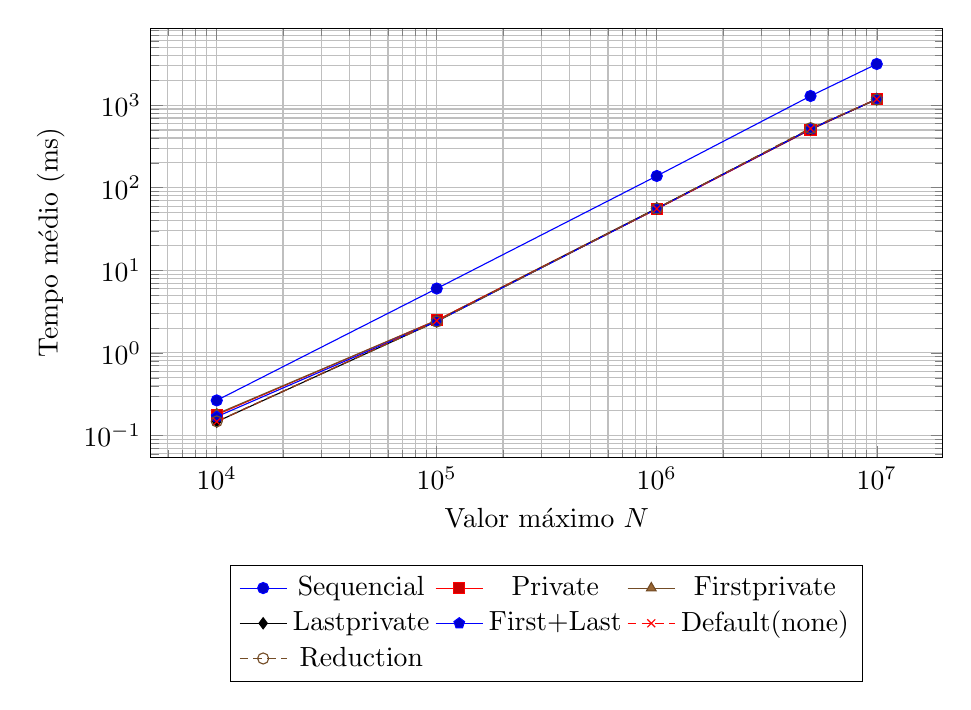
\begin{tikzpicture}
\begin{axis}[
    width=0.96\textwidth,
    height=0.58\textwidth,
    xmode=log,
    ymode=log,
    xlabel={Valor máximo \(N\)},
    ylabel={Tempo médio (ms)},
    grid=both,
    legend style={
        at={(0.5,-0.25)},
        anchor=north,
        legend columns=3
    },
    mark options={solid}
]

\addplot+[mark=*] coordinates {
    (10000,0.266162)
    (100000,6.022656)
    (1000000,138.899994)
    (5000000,1291.300023)
    (10000000,3152.100039)
};
\addlegendentry{Sequencial}

\addplot+[mark=square*] coordinates {
    (10000,0.178711)
    (100000,2.490625)
    (1000000,55.325007)
    (5000000,506.199956)
    (10000000,1183.499992)
};
\addlegendentry{Private}

\addplot+[mark=triangle*] coordinates {
    (10000,0.182812)
    (100000,2.480469)
    (1000000,56.550002)
    (5000000,506.450021)
    (10000000,1187.299991)
};
\addlegendentry{Firstprivate}

\addplot+[mark=diamond*] coordinates {
    (10000,0.147119)
    (100000,2.414062)
    (1000000,56.075001)
    (5000000,516.799998)
    (10000000,1176.650000)
};
\addlegendentry{Lastprivate}

\addplot+[mark=pentagon*] coordinates {
    (10000,0.168994)
    (100000,2.415626)
    (1000000,55.549985)
    (5000000,512.949979)
    (10000000,1182.150018)
};
\addlegendentry{First+Last}

\addplot+[mark=x] coordinates {
    (10000,0.147266)
    (100000,2.452344)
    (1000000,55.624998)
    (5000000,521.150029)
    (10000000,1181.499958)
};
\addlegendentry{Default(none)}

\addplot+[mark=o] coordinates {
    (10000,0.148340)
    (100000,2.403125)
    (1000000,55.975014)
    (5000000,526.800001)
    (10000000,1175.150001)
};
\addlegendentry{Reduction}

\end{axis}
\end{tikzpicture}

\caption{Tempo médio das versões de escopo de dados. As versões
funcionalmente incorretas são exibidas apenas para caracterização
experimental e não constituem soluções válidas para a contagem global.}
\label{fig:atvd07-data-sharing}
\end{figure}


\subsection{Comparação das políticas de escalonamento}

A Figura~\ref{fig:atvd07-scheduling} apresenta a comparação das cinco
políticas utilizando \texttt{reduction}.

\begin{figure}[htbp]
\centering

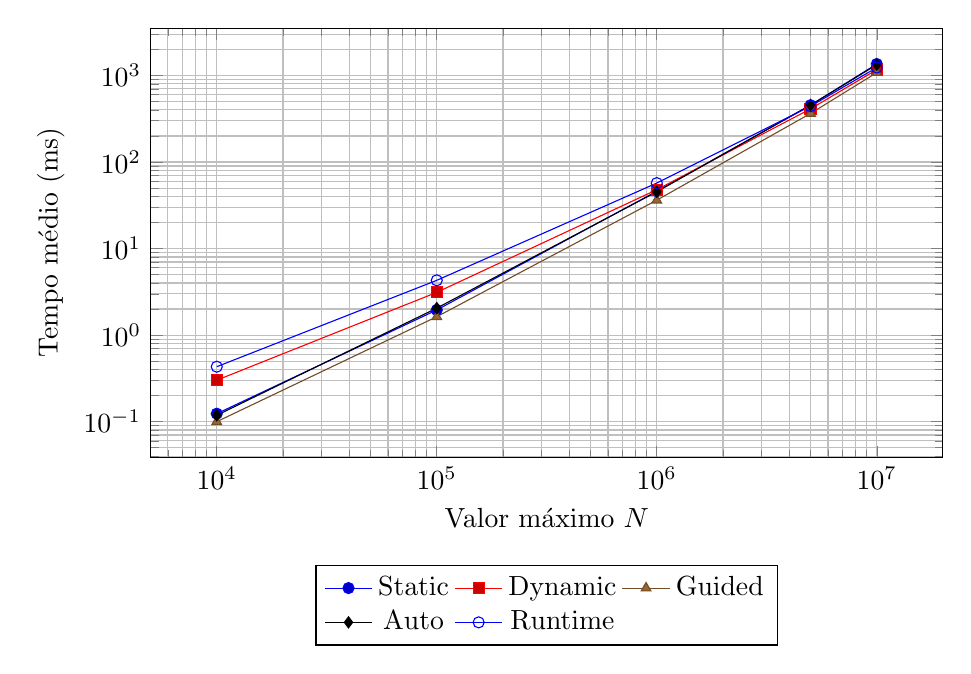
\begin{tikzpicture}
\begin{axis}[
    width=0.96\textwidth,
    height=0.58\textwidth,
    xmode=log,
    ymode=log,
    xlabel={Valor máximo \(N\)},
    ylabel={Tempo médio (ms)},
    grid=both,
    legend style={
        at={(0.5,-0.25)},
        anchor=north,
        legend columns=3
    },
    mark options={solid}
]

\addplot+[mark=*] coordinates {
    (10000,0.123535)
    (100000,1.951562)
    (1000000,45.974988)
    (5000000,453.599989)
    (10000000,1358.399987)
};
\addlegendentry{Static}

\addplot+[mark=square*] coordinates {
    (10000,0.301270)
    (100000,3.117969)
    (1000000,47.875017)
    (5000000,411.999989)
    (10000000,1169.500005)
};
\addlegendentry{Dynamic}

\addplot+[mark=triangle*] coordinates {
    (10000,0.099853)
    (100000,1.630468)
    (1000000,36.224997)
    (5000000,364.249992)
    (10000000,1079.549980)
};
\addlegendentry{Guided}

\addplot+[mark=diamond*] coordinates {
    (10000,0.118359)
    (100000,2.050000)
    (1000000,45.324993)
    (5000000,455.550027)
    (10000000,1332.999992)
};
\addlegendentry{Auto}

\addplot+[mark=o] coordinates {
    (10000,0.431250)
    (100000,4.295313)
    (1000000,57.125002)
    (5000000,441.750002)
    (10000000,1236.650026)
};
\addlegendentry{Runtime}

\end{axis}
\end{tikzpicture}

\caption{Tempo médio das políticas de escalonamento utilizando
\texttt{reduction}.}
\label{fig:atvd07-scheduling}
\end{figure}


\subsection{Speedup da redução em relação à execução sequencial}

A Figura~\ref{fig:atvd07-speedup} apresenta a aceleração obtida pela
implementação correta com \texttt{reduction + static} no primeiro
experimento.

\begin{figure}[htbp]
\centering

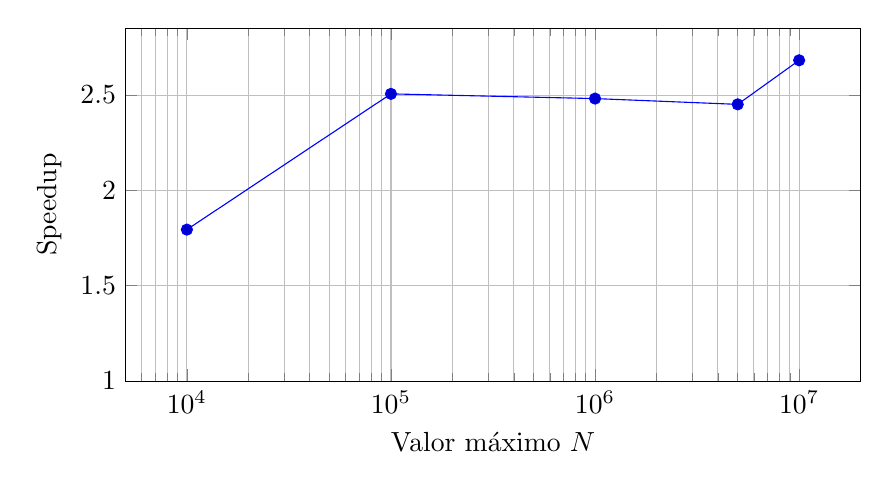
\begin{tikzpicture}
\begin{axis}[
    width=0.9\textwidth,
    height=0.5\textwidth,
    xmode=log,
    xlabel={Valor máximo \(N\)},
    ylabel={Speedup},
    ymin=1,
    grid=both,
    mark options={solid}
]

\addplot+[mark=*] coordinates {
    (10000,1.7943)
    (100000,2.5062)
    (1000000,2.4815)
    (5000000,2.4512)
    (10000000,2.6823)
};

\end{axis}
\end{tikzpicture}

\caption{Speedup da implementação \texttt{reduction + static} em relação à
versão sequencial no experimento de escopo de dados.}
\label{fig:atvd07-speedup}
\end{figure}


% ============================================================
\section{Análise e discussão}
\label{sec:atvd07-discussao}

\subsection{Escopo de dados não é equivalente a sincronização}

O primeiro experimento demonstrou que as cláusulas de escopo possuem
semânticas distintas e não podem ser utilizadas indistintamente para
resolver uma operação de acumulação global.

\texttt{private}, \texttt{firstprivate} e \texttt{lastprivate} tratam da
existência, inicialização ou transferência das cópias das variáveis.

Nenhuma delas, isoladamente, representa a soma das contribuições das
threads.


\subsection{Comportamento de \texttt{private}}

A versão \texttt{private} retornou zero para todos os valores de \(N\).

Isso não significa que as threads deixaram de realizar o trabalho.

Cada thread produziu sua própria contagem, mas as cópias privadas não foram
combinadas.

O contador externo permaneceu com o valor inicial:

\[
count=0.
\]

Portanto,

\[
\boxed{
\texttt{private}
\text{ fornece isolamento, não agregação}
}
\]


\subsection{Comportamento de \texttt{firstprivate}}

A versão \texttt{firstprivate} também retornou zero.

Cada cópia privada foi corretamente inicializada com o valor externo,
também igual a zero.

Entretanto, as cópias foram descartadas ao final da região paralela.

Assim,

\[
\boxed{
\texttt{firstprivate}
\text{ fornece inicialização privada, não agregação}
}
\]


\subsection{Comportamento de \texttt{lastprivate}}

A versão \texttt{lastprivate} retornou zero para todas as entradas.

Na implementação utilizada, \texttt{count} é reinicializado em cada
iteração antes da classificação do candidato.

Consequentemente, o valor propagado para fora da região corresponde à
classificação da última iteração lógica.

Todos os valores escolhidos para \(N\) são pares:

\[
10^4,\;
10^5,\;
10^6,\;
5\times10^6,\;
10^7.
\]

Logo, o último candidato de cada laço não é primo e o valor transferido foi

\[
0.
\]

O resultado evidencia que \texttt{lastprivate} não realiza uma redução.


\subsection{Comportamento de \texttt{firstprivate + lastprivate}}

Os resultados observados foram:

\[
279,\;
2199,\;
18260,\;
81795,\;
156318.
\]

Esses valores são inferiores à contagem global.

Com \texttt{schedule(static)}, as threads recebem blocos do espaço de
iterações.

A cópia privada associada à thread que executa a última iteração contém a
contagem acumulada naquela porção de trabalho.

\texttt{lastprivate} propaga essa cópia para a variável externa.

O resultado é, portanto, parcial e não representa:

\[
\sum_i C_i.
\]


\subsection{Comportamento de \texttt{default(none)}}

A versão \texttt{default(none)} produziu nesta execução os mesmos valores
numéricos observados em \texttt{firstprivate + lastprivate}.

Essa coincidência não indica equivalência semântica.

Na implementação com \texttt{default(none)}, \texttt{count} permanece
compartilhado e é atualizado simultaneamente pelas threads sem proteção.

Existe, portanto, uma condição de corrida.

Os valores obtidos devem ser interpretados apenas como o resultado
particular dessa execução.

Não existe garantia de que outra execução produza os mesmos números.

O resultado demonstra um ponto importante:

\[
\boxed{
\texttt{default(none)}
\text{ torna o escopo explícito, mas não garante sincronização}
}
\]


\subsection{Correção de \texttt{reduction}}

A implementação com redução reproduziu exatamente a referência sequencial
nos cinco valores avaliados.

Assim,

\[
C_{\mathrm{reduction}}(N)
=
C_{\mathrm{seq}}(N).
\]

A redução corresponde diretamente à operação necessária:

\[
C=
C_0+C_1+C_2+C_3.
\]

Por esse motivo, ela foi selecionada como base correta do segundo
experimento.


\subsection{Desempenho da versão com redução}

No primeiro experimento, a versão correta com redução apresentou speedups
entre aproximadamente

\[
1,79\times
\]

e

\[
2,68\times.
\]

Para o maior problema:

\[
N=10\,000\,000,
\]

os tempos foram:

\[
T_{\mathrm{seq}}
=
3152,100\,\mathrm{ms},
\]

e

\[
T_{\mathrm{reduction}}
=
1175,150\,\mathrm{ms}.
\]

O speedup correspondente foi:

\[
S
=
\frac{3152,100}{1175,150}
\approx
2,68.
\]

A utilização de quatro threads não implica um speedup de \(4\times\),
pois existem custos de criação e gerenciamento da região paralela,
sincronização, redução e compartilhamento dos recursos físicos da máquina.


\subsection{Correção das políticas de escalonamento}

Todas as cinco políticas produziram resultados numericamente idênticos à
referência sequencial.

Isso mostra que, uma vez resolvido corretamente o problema de agregação com
\texttt{reduction}, alterar a política de escalonamento modifica a forma de
distribuição do trabalho, mas não a semântica da computação.


\subsection{\texttt{guided} como melhor política observada}

A principal tendência do segundo experimento foi particularmente clara:
\texttt{guided} apresentou o menor tempo médio em todos os valores de \(N\).

Comparando com \texttt{static}, a redução aproximada do tempo foi:

\begin{center}
\begin{tabular}{|r|c|}
\hline
\textbf{\(N\)} & \textbf{Redução do tempo de \texttt{guided} vs.
\texttt{static}} \\
\hline
10\,000 & 19,2\% \\
100\,000 & 16,5\% \\
1\,000\,000 & 21,2\% \\
5\,000\,000 & 19,7\% \\
10\,000\,000 & 20,5\% \\
\hline
\end{tabular}
\end{center}

A vantagem permaneceu aproximadamente entre

\[
16,5\%
\]

e

\[
21,2\%.
\]

Esse comportamento é compatível com a irregularidade do problema.

A estratégia \texttt{guided} começa distribuindo blocos maiores, reduzindo o
custo de escalonamento, e progressivamente diminui esses blocos, melhorando
o balanceamento das partes restantes.


\subsection{Comportamento de \texttt{dynamic}}

Para os menores valores de \(N\), \texttt{dynamic} apresentou custo superior
a \texttt{static}.

Para \(N=10\,000\):

\[
T_{\mathrm{static}}
=
0,124\,\mathrm{ms},
\]

enquanto:

\[
T_{\mathrm{dynamic}}
=
0,301\,\mathrm{ms}.
\]

Quando a carga é pequena, o gerenciamento dinâmico representa uma fração
significativa do tempo.

Entretanto, para cargas maiores o comportamento se inverteu.

Para

\[
N=5\,000\,000,
\]

foram observados:

\[
T_{\mathrm{static}}
=
453,600\,\mathrm{ms},
\]

e

\[
T_{\mathrm{dynamic}}
=
412,000\,\mathrm{ms}.
\]

Para

\[
N=10\,000\,000,
\]

foram observados:

\[
T_{\mathrm{static}}
=
1358,400\,\mathrm{ms},
\]

e

\[
T_{\mathrm{dynamic}}
=
1169,500\,\mathrm{ms}.
\]

Assim, o ganho decorrente de melhor balanceamento passou a compensar o
overhead adicional à medida que a carga cresceu.


\subsection{Comportamento de \texttt{static}}

A política estática apresentou bom desempenho principalmente para as cargas
menores.

Seu principal benefício é o baixo custo de distribuição.

O problema, entretanto, apresenta iterações com custos diferentes.

Um bloco com maior quantidade de candidatos computacionalmente caros pode
fazer com que uma thread continue trabalhando depois que outras já tenham
terminado.

Esse desequilíbrio ajuda a explicar por que \texttt{guided} passou a
apresentar vantagem consistente.


\subsection{Comportamento de \texttt{auto}}

Os tempos de \texttt{auto} permaneceram próximos aos observados para
\texttt{static}:

\[
\begin{array}{c|cc}
N & T_{\mathrm{static}} & T_{\mathrm{auto}}\\
\hline
10^4 & 0,124 & 0,118\\
10^5 & 1,952 & 2,050\\
10^6 & 45,975 & 45,325\\
5\times10^6 & 453,600 & 455,550\\
10^7 & 1358,400 & 1333,000
\end{array}
\]

Esses resultados mostram um perfil temporal semelhante.

Entretanto, os tempos não permitem afirmar qual política interna foi
selecionada pela implementação OpenMP.

A conclusão possível é apenas que \texttt{auto} apresentou, neste ambiente,
desempenho próximo ao observado para \texttt{static}.


\subsection{Comportamento de \texttt{runtime}}

A política \texttt{runtime} foi configurada como:

\[
\texttt{dynamic,1}.
\]

Para cargas pequenas, apresentou o maior tempo entre as estratégias
avaliadas.

Para

\[
N=10\,000,
\]

o resultado foi:

\[
0,431\,\mathrm{ms}.
\]

Para os maiores tamanhos, a diferença relativa foi reduzida.

Em

\[
N=10\,000\,000,
\]

o tempo foi:

\[
1236,650\,\mathrm{ms}.
\]

Esse valor foi inferior a \texttt{static} e \texttt{auto}, mas superior a
\texttt{dynamic} e \texttt{guided}.

O resultado evidencia que a flexibilidade de selecionar a política em tempo
de execução também pode envolver custos adicionais e que o desempenho
observado deve ser analisado junto à configuração efetivamente utilizada.


\subsection{Diferença entre as duas medições de \texttt{static}}

A versão \texttt{reduction} do experimento de escopo utiliza
\texttt{schedule(static)}, e a política \texttt{static} aparece novamente no
segundo experimento.

Os tempos não foram idênticos.

Por exemplo, para

\[
N=10\,000\,000,
\]

foram obtidos:

\[
1175,150\,\mathrm{ms}
\]

no primeiro bloco e

\[
1358,400\,\mathrm{ms}
\]

no segundo.

Isso não caracteriza uma inconsistência funcional.

Os dois valores resultam de blocos de benchmark realizados em momentos
diferentes durante a mesma execução.

Fatores como estado térmico, frequência da CPU, atividade do sistema
operacional e histórico de execução podem afetar tempos absolutos.

Por esse motivo, as comparações principais foram realizadas
\textbf{dentro de cada experimento}, e não misturando valores pertencentes
a blocos diferentes.


% ============================================================
\section{Limitações}
\label{sec:atvd07-limitacoes}

\subsection{Execução em uma única máquina}

Os resultados representam o ambiente utilizado na atividade.

Processadores com outras arquiteturas, quantidades de núcleos, hierarquias
de cache ou runtimes OpenMP podem apresentar relações diferentes entre as
estratégias.


\subsection{Quantidade fixa de threads}

Foram utilizadas quatro threads em todas as medições.

Portanto, os resultados não constituem um estudo de escalabilidade em
função da quantidade de threads.


\subsection{Ausência de afinidade explícita}

Não foi implementado controle explícito de afinidade das threads.

O posicionamento nos processadores lógicos ficou sob responsabilidade do
runtime e do sistema operacional.


\subsection{Sensibilidade da média a outliers}

A média aritmética é sensível a valores extremos.

Durante uma execução anterior, interrompida em condições inadequadas de
energia, foi observada uma medição anômala de grande magnitude.

Essa execução foi descartada e não faz parte dos resultados apresentados
neste capítulo.

A coleta final foi realizada integralmente e não apresentou aquela
anomalia.

Ainda assim, a escolha da média, necessária para acompanhar o objetivo da
atividade, continua mais sensível a interferências externas do que a
mediana utilizada na Atividade 5.


\subsection{Versão \texttt{default(none)} com condição de corrida}

A implementação \texttt{default(none)} contém deliberadamente uma atualização
concorrente não sincronizada.

Seus valores servem apenas para demonstrar a diferença entre escopo explícito
e sincronização.

Eles não devem ser interpretados como resultados numéricos reproduzíveis.


\subsection{Versões funcionalmente incorretas}

Os tempos de \texttt{private}, \texttt{firstprivate},
\texttt{lastprivate}, \texttt{firstprivate + lastprivate} e
\texttt{default(none)} foram medidos para caracterizar o experimento.

Entretanto, comparar esses tempos diretamente com \texttt{reduction} como
se fossem soluções concorrentes seria inadequado, pois não calculam a mesma
resposta global.


\subsection{Trabalho auxiliar das versões privadas}

As versões \texttt{private} e \texttt{firstprivate} utilizam uma estrutura
auxiliar para manter observáveis as contagens privadas.

Esse mecanismo impede que a computação seja eliminada pelo compilador, mas
introduz pequeno custo adicional que faz parte de seus tempos medidos.


\subsection{Calibração comum}

O número de repetições internas foi definido a partir da versão sequencial e
da versão \texttt{reduction + static}.

A mesma quantidade foi reutilizada em todas as estratégias.

Assim, uma configuração significativamente mais rápida pode produzir um
lote inferior ao alvo nominal de \(100\,\mathrm{ms}\).

Essa decisão foi adotada para utilizar a mesma quantidade de repetições nas
versões comparadas.


\subsection{Tamanho dos blocos}

Não foi realizada uma exploração sistemática de diferentes
\textit{chunk sizes}.

Consequentemente, as conclusões dizem respeito às políticas avaliadas com
as configurações utilizadas, e não à totalidade das combinações possíveis
de política e tamanho de bloco.


\subsection{\texttt{runtime} não constitui uma política independente}

\texttt{schedule(runtime)} obtém sua configuração em tempo de execução.

Nesta atividade foi utilizado:

\[
\texttt{dynamic,1}.
\]

Portanto, os resultados da coluna \texttt{runtime} devem ser interpretados
como o comportamento da implementação utilizando essa configuração por meio
do mecanismo \texttt{runtime}, e não como um sexto algoritmo de
escalonamento independente.


\subsection{Ausência de medidas de dispersão}

Foram realizadas vinte medições e reportadas suas médias.

O programa não exportou desvio-padrão, intervalo de confiança ou outras
medidas de dispersão.

A análise está, portanto, baseada nos tempos médios observados.


% ============================================================
\section{Conclusões da atividade}
\label{sec:atvd07-conclusao}

A atividade demonstrou que mecanismos de escopo de dados e mecanismos de
sincronização possuem responsabilidades distintas em OpenMP.

As cláusulas \texttt{private}, \texttt{firstprivate} e
\texttt{lastprivate} alteram a forma como uma variável existe ou é
transferida dentro de uma região paralela, mas não realizam automaticamente
a agregação necessária à contagem global de números primos.

Da mesma forma, \texttt{default(none)} torna a classificação das variáveis
explícita, mas não elimina uma condição de corrida quando uma variável
compartilhada continua sendo atualizada sem sincronização.

A cláusula

\begin{verbatim}
reduction(+:count)
\end{verbatim}

foi a implementação paralela do primeiro experimento que reproduziu
corretamente a referência sequencial em todos os tamanhos.

Os speedups observados para essa versão em relação à sequencial variaram
aproximadamente entre

\[
1,79\times
\]

e

\[
2,68\times.
\]

Depois de estabelecida uma implementação funcionalmente correta, a
comparação das políticas de escalonamento mostrou que todas preservaram a
contagem correta, mas apresentaram diferenças significativas de desempenho.

A política \texttt{guided} apresentou o menor tempo médio para todos os
tamanhos avaliados.

Sua vantagem sobre \texttt{static} ficou aproximadamente entre

\[
16,5\%
\]

e

\[
21,2\%.
\]

O resultado é compatível com a natureza irregular do teste de primalidade:
a política guiada consegue combinar blocos inicialmente maiores com
redistribuição progressivamente mais fina do trabalho.

\texttt{dynamic} mostrou claramente o trade-off entre overhead e
balanceamento: apresentou desempenho inferior a \texttt{static} nas cargas
menores, mas passou a superá-lo nos dois maiores tamanhos.

A atividade evidencia, portanto, dois princípios importantes de HPC:

\[
\boxed{
\text{primeiro garantir correção, depois otimizar desempenho}
}
\]

e

\[
\boxed{
\text{a forma como o trabalho é distribuído pode ser tão importante
quanto a criação das threads}
}
\]


% ============================================================
\section{Síntese}
\label{sec:atvd07-defesa}

Os principais pontos para defesa oral da atividade são:

\begin{enumerate}

    \item \textbf{Continuidade da atividade anterior:}
    a Tarefa 7 reutiliza a contagem de primos da Tarefa 5 e mantém o mesmo
    algoritmo de primalidade.

    \item \textbf{Dois experimentos:}
    primeiro foram estudadas cláusulas de escopo de dados; depois foram
    estudadas políticas de escalonamento.

    \item \textbf{Variável crítica:}
    o problema central é o contador global de números primos.

    \item \textbf{\texttt{private}:}
    cada thread possui sua própria cópia, mas as cópias não são somadas.
    Por isso o contador externo permaneceu zero.

    \item \textbf{\texttt{firstprivate}:}
    as cópias começam com o valor inicial correto, mas continuam sendo
    descartadas ao final. O resultado também foi zero.

    \item \textbf{\texttt{lastprivate}:}
    apenas o valor da última iteração lógica é propagado. Como todos os
    valores de \(N\) eram pares, o resultado observado foi zero.

    \item \textbf{\texttt{firstprivate + lastprivate}:}
    houve inicialização das cópias e propagação de uma delas, mas não soma
    global. Foram obtidos apenas resultados parciais.

    \item \textbf{\texttt{default(none)}:}
    obriga a declaração explícita do escopo, mas não sincroniza a variável.
    O contador compartilhado continuou sujeito a uma data race.

    \item \textbf{Coincidência de resultados:}
    \texttt{default(none)} produziu nesta execução os mesmos valores de
    \texttt{firstprivate + lastprivate}, mas isso não significa equivalência
    entre as duas construções.

    \item \textbf{\texttt{reduction}:}
    foi a implementação paralela que agregou corretamente as contagens
    locais e reproduziu a referência sequencial em todos os casos.

    \item \textbf{Critério de escolha:}
    uma versão incorreta não pode ser considerada melhor apenas por ser mais
    rápida. A correção foi verificada antes do desempenho.

    \item \textbf{Speedup da redução:}
    em relação à versão sequencial, foram observados aproximadamente
    \(1,79\times\), \(2,51\times\), \(2,48\times\),
    \(2,45\times\) e \(2,68\times\).

    \item \textbf{Segundo experimento:}
    todas as versões de scheduling utilizaram \texttt{reduction}, para que
    somente a distribuição do trabalho fosse alterada.

    \item \textbf{Schedules avaliados:}
    \texttt{static}, \texttt{dynamic}, \texttt{guided}, \texttt{auto} e
    \texttt{runtime}.

    \item \textbf{Correção dos schedules:}
    todos produziram exatamente as mesmas contagens da referência
    sequencial.

    \item \textbf{Melhor resultado:}
    \texttt{guided} apresentou o menor tempo médio em todos os cinco
    tamanhos testados.

    \item \textbf{Vantagem de \texttt{guided}:}
    em relação a \texttt{static}, a redução de tempo ficou aproximadamente
    entre \(16,5\%\) e \(21,2\%\).

    \item \textbf{Explicação para \texttt{guided}:}
    o teste de primalidade possui custo irregular; guided utiliza blocos
    maiores inicialmente e reduz o tamanho dos blocos progressivamente,
    equilibrando overhead e distribuição de carga.

    \item \textbf{\texttt{dynamic}:}
    foi mais caro para problemas pequenos, mas superou \texttt{static} para
    \(N=5\times10^6\) e \(N=10^7\), quando o benefício do balanceamento
    passou a compensar seu overhead.

    \item \textbf{\texttt{auto}:}
    apresentou tempos próximos aos de \texttt{static}, mas os resultados
    não permitem afirmar qual estratégia interna foi selecionada.

    \item \textbf{\texttt{runtime}:}
    foi configurado explicitamente como \texttt{dynamic,1}; portanto seus
    resultados devem ser interpretados considerando essa configuração.

    \item \textbf{Metodologia:}
    foram utilizadas quatro threads, três warm-ups, vinte medições,
    rotação da ordem das versões e média aritmética.

    \item \textbf{Temporização:}
    foi utilizado \texttt{omp\_get\_wtime()} e repetição interna calibrada
    para melhorar a medição das cargas pequenas.

    \item \textbf{Conclusão principal:}
    escopo, sincronização e escalonamento resolvem problemas diferentes.
    Uma implementação paralela correta exige primeiro controlar a semântica
    dos dados e somente depois otimizar a distribuição do trabalho.

\end{enumerate}
